\begin{figure*}
\resizebox{\textwidth}{!}{
\begin{tabular}{ccc}
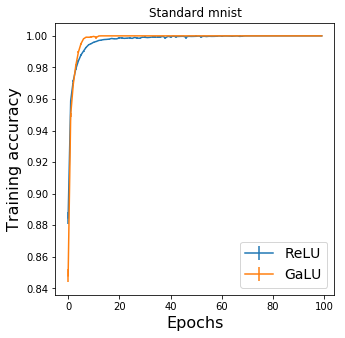
\includegraphics[scale=0.1]{figs/mnist-normal-opt.png}
&
%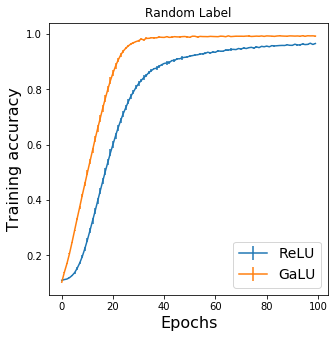
\includegraphics[scale=0.1]{figs/mnist-rand-label.png}
%&
%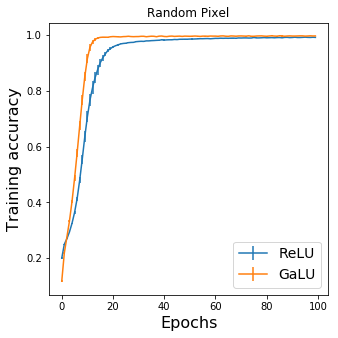
\includegraphics[scale=0.1]{figs/mnist-rand-pixel.png}
%&
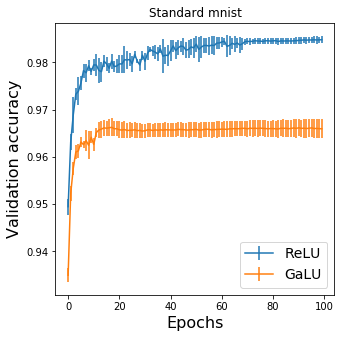
\includegraphics[scale=0.1]{figs/mnist-normal-gen.png}
&
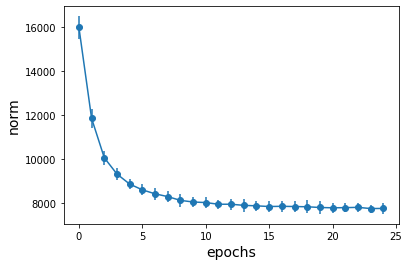
\includegraphics[scale=0.125]{figs/path-gram.png}
	\end{tabular}
}
\caption{First two plots from the left show optimisation and generalisation in ReLU and GaLU networks for standard MNIST. The right most plot shows $\nu_t=y^\top (\widehat{M}_t)^{-1}y$, where $M_t=\Phi_t^\top \Phi_t$.}
\label{fig:galu-relu}
\end{figure*}
